\documentclass[a4paper,ngerman,12pt]{scrartcl}

\usepackage[utf8]{inputenc}
%\usepackage[ansinew]{inputenc}

\usepackage[ngerman]{babel}

\usepackage{amsmath,amsthm,amssymb,stmaryrd,color,graphicx}
\usepackage{setspace}
\usepackage{bussproofs}
\usepackage{array}
\usepackage{comment}
\usepackage{wrapfig}

\usepackage{enumitem}

\usepackage{units}

\usepackage[protrusion=true,expansion=true]{microtype}

\usepackage{lmodern}

\usepackage{hyperref}
\usepackage{cleveref}

\newcommand{\RR}{\mathbb{R}}
\newcommand{\CC}{\mathbb{C}}
\newcommand{\ZZ}{\mathbb{Z}}
\newcommand{\NN}{\mathbb{N}}
\newcommand{\QQ}{\mathbb{Q}}

\setlength\parskip{\medskipamount}
\setlength\parindent{0pt}

\theoremstyle{definition}
\newtheorem{defn}{Definition}[]
\newtheorem{axiom}[defn]{Axiom}
\newtheorem{bsp}[defn]{Beispiel}

\theoremstyle{plain}
\newtheorem{prop}[defn]{Proposition}
\newtheorem{motto}[defn]{Motto}
\newtheorem{wunder}[defn]{Wunder}
\newtheorem{ueberlegung}[defn]{Überlegung}
\newtheorem{lemma}[defn]{Lemma}
\newtheorem{kor}[defn]{Korollar}
\newtheorem{hilfsaussage}[defn]{Hilfsaussage}
\newtheorem{satz}[defn]{Satz}
\newtheorem{frage}[defn]{Frage}

\theoremstyle{remark}
\newtheorem{bem}[defn]{Bemerkung}
\newtheorem{aufg}[defn]{Aufgabe}

\newtheorem*{antwort}{Antwort}

\newlength{\aufgabenskip}
\setlength{\aufgabenskip}{1.4em}
\newcounter{aufgabennummer}
\newenvironment{aufgabe}[1]{
	\addtocounter{aufgabennummer}{1}
	\textbf{Aufgabe \theaufgabennummer.} \emph{#1} \par
}{\vspace{\aufgabenskip}}

\clubpenalty=10000
\widowpenalty=10000
\displaywidowpenalty=10000

\setlength\unitlength{1cm}

\usepackage{tikz}

\RequirePackage{geometry}
\geometry{textwidth=16.0cm,textheight=24.5cm,footskip=1.5cm}

\usepackage{todonotes}


\begin{document}
	
\begin{picture}(0,0)
\put(0,-0.5){%
	
\includegraphics[scale=0.1]{logo-ifm}
}
\put(14.0,-3.5){%
	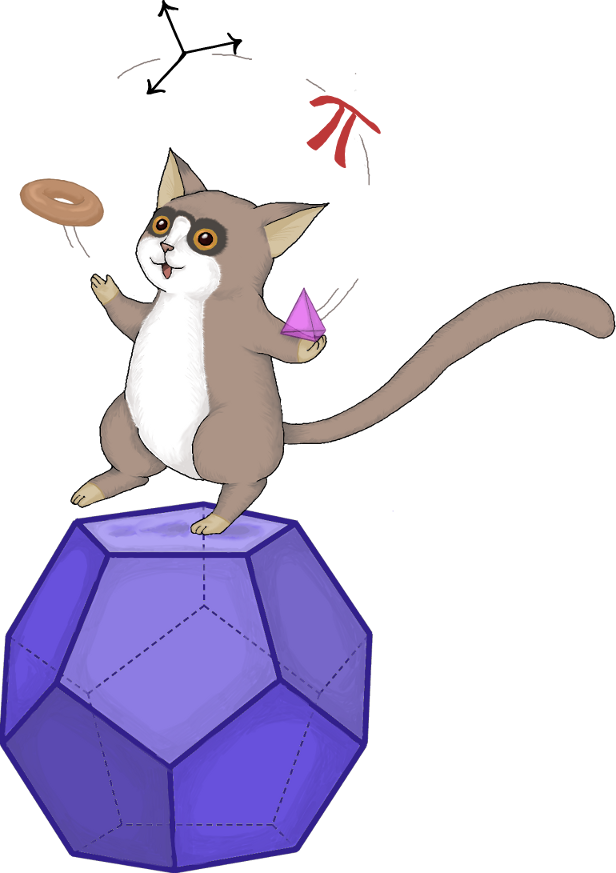
\includegraphics[scale=0.17]{cover}
}
\end{picture} 
	
\vspace{6em}

\begin{center}\Large{Vierter Korrespondenzbrief}\end{center}

\section*{Erste Beweise mit Induktion}

In diesem Brief werden wir eine besondere, in der Mathematik sehr oft genutzte Beweistechnik kennen lernen: Den \emph{Beweis durch Induktion}. Eine Besonderheit dieser Beweistechnik ist, dass man mit ihr nicht nur eine Aussage, sondern gleich unendlich viele Aussagen auf einmal zeigen kann! 

Vor kurzem habe ich mal wieder mei  Sparschein geleert um es zur Bank zu bringen. Davor wollte ich aber natürlich wissen, wie viel Geld sich überhaupt darin befunden hatte. Und um mir das Zählen zu erleichtern (und vielleicht auch, weil mir gerade ein wenig langweilig war) habe ich die Münzen zu einem Muster zusammengelegt:

\missingfigure{Die ersten vier(?) zentrierten Viereckszahlen}

\begin{aufgabe}{}
	Erkennst du das Schema, nach dem ich dieses Muster gebaut habe? Kannst du das nächste Viereck zeichnen?
\end{aufgabe}

Während ich also immer größere Vierecke gelegt habe, ist mir das folgende aufgefallen: Die Zahl an Münzen, die ich für ein Viereck benötige, scheint immer eine ungerade Zahl zu sein: Für das erste $1$, beim zweiten $5$, beim dritten $13$, beim vierten $25$, beim fünften \underline{\phantom{ 41 }}, \dots

Ob das wohl für alle solchen Vierecke stimmt? Ich habe noch ein paar weitere solchen Vierecke gelegt, und für tatsächlich habe ich für jedes eine ungerade Anzahl an Münzen gebraucht. Aber irgendwann sind mir natürlich die Münzen ausgegangen. Wie kann ich nun also herausfinden, ob meine Vermutung wirklich für \emph{alle} solche Vierecke gilt?

Wir haben nun also für ein paar kleine Beispiele gesehen, dass die Aussage \glqq Für ein (zentriertes) Viereck benötigt man eine ungerade Zahl an Münzen.\grqq{} für diese stimmt. Wir können nun aber nicht \emph{alle} möglichen Vierecke durchprobieren und für jedes einzelne prüfen, ob die Aussage auch für diese stimmt.

Ein ähnliches Problem hatten wir zu Beginn dieses Schuljahres schon einmal in einem Zirkelbrief? Erinnerst du dich noch an den Brief mit den Unmöglichkeitsbeweisen? Den Tetrominos, den Schachbrettern und den Chamäleons? 

\missingfigure{Kleines Bild von Tetrominos, Schachbrettern und Chamäleons?}

Darin hatten wir doch ein ganz ähnliches Problem: Wir hatten zum Beispiel eine Menge verschiedenfarbiger Chamäleons, die ihre Farbe nach einem bestimmten Muster ändern, wenn sie sich treffen. Wir wollten nun zeigen, dass wir nie gleich viele Chamäleons jeder Farbe bekommen können.


Erstes Beispiel: Alle zentrierten Viereckszahlen sind ungerade - entspricht unendlich vielen Aussagen: Die erste Viereckszahl ist ungerade, die zweite, die dritte, ...

Vorgehen: Klar für kleine Zahlen, um es auch für größere Zahlen zu zeigen, zeigen wir, dass die Eigenschaft erhalten bleibt, wenn wir das Viereck um eine "Stufe" größer machen (vergleiche 1. Korrespondenzbrief zu Invarianten).

Weiteres dazu: Beweise n-te Viereckszahl ist $2n^2-2n+1$.

Beweise für diese Formel: Zahl ist für alle $n$ ungerade (vllt. vor dem Beweis des Zusammenhangs zur Viereckszahl?)

Beweise: Jede Viereckszahl ist Summe zweier aufeinander folgender Quadratzahlen (evtl. auch durch Bild?)

\hrule

Formalisierung: Induktionsanfang + Induktionsvoraussetzung + Induktionsschritt

\hrule

Beweise: Die Länge der Kochschen Schneeflocke ist unendlich bzw. besser: Nach $n$ Schritten hat sie Länge $> n$

Analog: Die Fläche des Sierpinski-Dreiecks ist $0$

\hrule

Josephus-Problem

\hrule

Beweise über Bäume? Evtl. als "echte" Bäume beschreiben und nur kurzer Hinweis auf Graphentheorie?

\hrule

Induktion verwendet man auch für Korrektheitsbeweise von Computerprogrammen:

Beispiel: Quadratzahl $x^2$ berechnen als $x+x-1 +x-1+x-2 + \dots +1$ - evtl. dargestellt als Flussdiagramm (rekursives Programm!)

Aufgabe?

Euklidischer Algorithmus? Verweis auf zweiten Brief

\hrule

\begin{bem}
Lauter Aussagen über natürliche Zahlen. Dies liegt daran, dass die natürlichen Zahlen selbst mit Hilfe von Induktion definiert sind. Verweis auf Peano-Axiome
\end{bem}

\end{document}